\section{Chronologie}
\label{sec:chronologie}

	Cette séparation des tâches nous a permis de réaliser un diagramme de Gantt du projet, avec des ressources affectées pour chaque tâche. Retranscrire exactement le diagrammede Gantt ne rendrait pas celui-ci très lisible, nous avons donc réalisé grâce à l'outil disponible sous Microsoft Project une frise chronologique qui reprend dans les grandes lignes ce dernier. Celui-ci est cependant disponible en annexe pour voir la liste entière de toutes les tâches du projet.

	\begin{figure}[H]
        \centering
        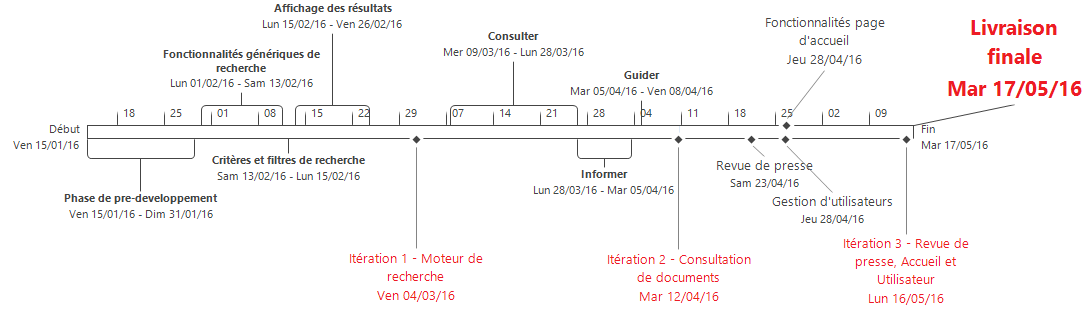
\includegraphics[width=1.3\textwidth, angle=90]{figure/frise.png}
            \caption{Frise chronologique représentant l'ensemble de la planification}
            \label{fig:frise}
    \end{figure}